\documentclass[a4paper]{report}
\usepackage{amsmath}
\usepackage{blindtext}
\usepackage{blindtext}
\usepackage[utf8]{inputenc}
\usepackage{graphicx}
\usepackage{appendix}




%front page:
\usepackage[T1]{fontenc}
\usepackage{xcolor}

%for MATLAB code:
\usepackage{listings}

\usepackage{geometry}
\geometry{a4paper, margin=1in}


\begin{document}
	
\begin{titlepage}

		\centering
		\vspace*{5\baselineskip}
		\Huge
		Finite Elements
		\\[2\baselineskip]
		\normalsize
		Rick Koster\\
		Ruben Termaat\\
		\today
		\vfill
		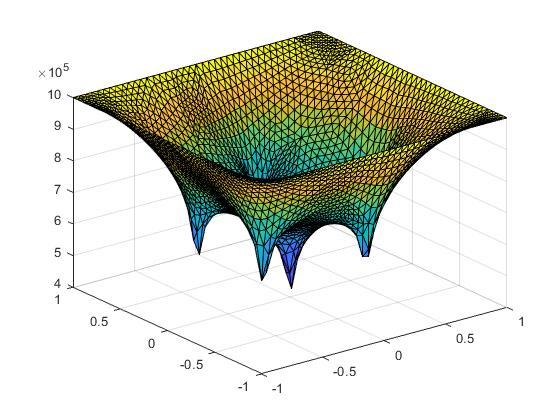
\includegraphics[width=15cm]{3Dv.jpg}
		\vfill
	
\end{titlepage}
	
\clearpage\mbox{}\clearpage

\tableofcontents


\chapter{1D-case}



On the 1D interval of $x = [0,1]  $, we consider a steady-state convection-diffusion-reaction equation, with homogeneous Neumann boundary conditions. The following equations apply to this domain:

\begin{equation}
\begin{cases} 
-D\triangle u + \lambda u = f(x),\\ -D\frac{du}{dx}(0) = 0 ,\\ -D\frac{du}{dx}(1) = 0
\end{cases} 
\end{equation}
\bigskip

In this report $\triangle$ denotes the laplacian operator. The function f(x) is a given funtion, where D and $\nabla$ are positive real constants. In order to solve this boundary value problem (BVP), first the interval is divided in n-1 elements(n = positive integer). This results in the domain being divided in elements: $e_i = [x_i, x_{i-1}]$ where $i={1,2,..,n}$. 

In order to solve this BVP, the solutions for the given equations will first be calculated and then computed using MATLAB codes.


\section{Boundary value problem 1D}
\vspace{5mm}

In order to find the Weakform of the given equations(1.1), both sides are multiplied by a test function  $\phi(x)$ and then integrate both sides over the domain $\Omega$. In the equations  $\phi(x)$ is written as $\phi$


\begin{equation}
	 \int_{\Omega} \phi(-D\triangle u + \lambda u )d\Omega = \int_{\Omega} \phi f(x) d\Omega 
\end{equation}	
\smallskip

Now by rewriting and then using partial integration the following equation can be found:


\begin{equation}
	\int_{\Omega} (\nabla\cdot(-D\phi\cdot\nabla u) + D\nabla\phi\nabla u +\phi \lambda u) d\Omega = \int_{\Omega} \phi f(x) d\Omega 
\end{equation}
\smallskip

Applying Gauss on the first term on the left side of equation(1.3):


\begin{equation}
	\int_{\Omega}  \vec{n}\cdot(-D\phi \nabla u) d\tau + \int_{\Omega}  (D\nabla\phi\cdot\nabla u +\phi\lambda u )d\Omega = \int_{\Omega} \phi f(x) d\Omega 
\end{equation}
\smallskip

Using the boundary conditions from equations(1.1) the boundary integral equals to 0 and then the following weak formulation(WF) is found: \vspace{5mm}


(WF): \begin{equation}
\begin{cases} 
	$find u $\epsilon \sum =\{u$ $ smooth\}$ Such that:$ \\ \int_{\Omega}  (D\nabla\phi\cdot\nabla u +\phi\lambda u )d\Omega = \int_{\Omega} \phi f(x) d\Omega \\ \forall\phi $ $ \in\sum 
\end{cases}\  
\end{equation}

\bigskip
The next step is to substitute the Galerkin equations into the found diferential equation, where u is replaced by $ \sum_{j=1}^{n}c_i\phi_j $ and  $\phi(x)=\phi_i(x)$ with $i = [1,..,n]$. Filling this in equation (1.5) the following equation is found:

\begin{equation}
	\sum_{j=1}^{n}c_i\int_{0}^{1} (D\nabla\phi_i\cdot\nabla\phi_j +\lambda\phi_i\phi_j )d\Omega = \int_{0}^{1} \phi_i f(x) d\Omega
\end{equation}
\medskip

Which is of the form of $ S\vec{c} = \vec{f} $

\section{Element matrix}
Now the found Galerkin equations can be used to compute $ S_{ij}$  the element matrix, over a generic line element $ e_i$.

\begin{equation}
S\vec{c}=	\sum_{j=1}^{n}c_i\int_{0}^{1} (D\nabla\phi_i\cdot\nabla\phi_j +\lambda\phi_i\phi_j )d\Omega
\end{equation}

\begin{equation}
S_{ij} =\sum_{l=1}^{n-1} S^{e_k}_{ij} 
\end{equation}
\medskip

Now to solve S we solve the following equation, over the internal line element.

\begin{equation}
S^{e_k}_{ij} = -D\int_{e_k}\nabla\phi_i\cdot\nabla\phi_j d\Omega+\lambda\int_{e_k}\phi_i\phi_j dx
\end{equation}


\section{Element vector}
Again the found Galerkin Equations(1.6) are used in order to compute the element vector $f_i$ over a generic line-element.

\begin{equation}
f^{e_k}_i = \int_{e_k}\phi_i f dx
\end{equation}

\begin{equation}
	f^{e_k}_i =\frac{\lvert x_k-x_{k-1}\lvert}{(1+1+0)!}f(\vec{x}) =\frac{\lvert x_k-x_{k-1}\lvert}{2}
	\begin{bmatrix} f^{e_n}_{k-1}\\ f^{e_n}_{k}
	\end{bmatrix}
\end{equation}







\section{Boundary value problem 1D MATLAB routine}

\subsection{mesh and elmat code}
The first step in order to solve the BVP is to write a MATLAB routine that generates an equidistant distrubition of points over the given interval of $[0,1]$(generate a mesh with n-1 elements).

\begin{lstlisting}
	function [ x ] = GenerateMesh(int, N_elem)
	%GenerateMesh Creates a mesh for 1D problems
	
	
	% int = [0,1];
	% N_elem = 100;
	
	x = linspace(int(1,1),int(1,2),N_elem);
	
\end{lstlisting}
	
Using the codes to generate a mesh and the elmat, it is easier to use this 1D problem and adapt to a higher dimensional problem. The next step is to write a code that generates a two dimensional array, called the elmat.

\begin{lstlisting}
	function [ elmat ] = GenerateTopology( N_elem )
	%GenerateTopology Creates the topology for a 1D problem given mesh 'x'.
	
	% global N_elem
	elmat = zeros(N_elem,2);
	elmat(i,1) = i;
	elmat(i,2) = i + 1;

\end{lstlisting}

\subsection{Element matrix}

Now that the base MATLAB codes are made the element matrix and element vector codes can be written. The first step in this process is, is to compute the element matrix $S_{elem}$.

\begin{lstlisting}
	function [ Selem ] = GenerateElementMatrix( k, elmat, D, lambda, mesh)
	%GenerateElementMatrix Creates element matrix S_ek
	
	
	Selem = zeros(2,2);
	
	i = elmat(k,1);
	j = elmat(k,2);
	
	x1 = mesh(i);
	x2 = mesh(j);
	
	element_length = abs(x1-x2);
	
	slope = 1/element_length; 
	
	for m = 1:2
		for n = 1:2
			if m == n
				Selem(m,n) = element_length*((-1)^(abs(m-n))*D*slope^2
				+ (2)*lambda/6);
			else
				Selem(m,n) = element_length*((-1)^(abs(m-n))*D*slope^2
				+ (1)*lambda/6);
			end
			end
	
		end
	
	end
\end{lstlisting}

\bigskip




\subsection{Assemble matrix S}
To generate a n-by-n matrix S, the sum over the connections of the vertices in each element matrix, over all elements has to be calculated. The following code computes this matrix:

\begin{lstlisting}
	function [ S ] = AssembleMatrix( N_elem, int, lambda, D)
	% global N_elem 
	
	elmat = GenerateTopology(N_elem);
	
	S = zeros(N_elem,N_elem);
	
	for i = 1:N_elem-1
		Selem = GenerateElementMatrix(i, elmat, int, N_elem, D, lambda);
		for j = 1:2
			for k = 1:2
				S(elmat(i,j), elmat(i,k)) =
				S(elmat(i,j), elmat(i,k)) +	Selem(j,k);
			end
		end
	end


\end{lstlisting}



All the previous code will generate a large matrix S, from the element matrices $S_{elem}$ over each element.\\



\subsection{Element vector MATLAB routine}

The next step In order to solve the equation $S\vec{c}=F$ is to create a code to generate the element vector. This element vector provides information about note $i$ and node $i+1$, which are the vertices of element $e_i$.\\



\begin{lstlisting}
	function [ felem ] = GenerateElementVector( i, elmat, mesh )
	%GenerateElementVector Creates element vector f_ek
	
	
	felem = [0;0];
	
	k1 = elmat(i,1);
	k2 = elmat(i,2);
	
	x1 = mesh(k1);
	x2 = mesh(k2);
	
	element_length = abs(x1-x2);
	
	felem = (element_length/2*arrayfun(@functionBVP,[x1,x2]))';
	
	end
\end{lstlisting}

\smallskip

To generate the vector f, the sum over the connections of the vertices in each element matrix, over all elements $i\,\epsilon\, \{1,...,n-1\}$  has to be calculated. 

\bigskip

	
\begin{lstlisting}
	function [ f ] = AssembleVector( N_elem, int, lambda, D )
		
	f = zeros(N_elem,1);
	elmat = GenerateTopology(N_elem);
		
	for i = 1:N_elem-1
		felem = GenerateElementVector(i, elmat, int, N_elem);
		for j = 1:2
			f(elmat(i,j)) = f(elmat(i,j)) + felem(j);
		end
	end
\end{lstlisting}	




\subsection{Computing S and f}

Now if the previous matlab codes are run the following happens. Firstly a mesh and 1D topology is build, which is needed for the S matrix and f vector. The second step is to calculate the S matrix and f vector through the found equations of section 1.2 and 1.3. The final step is to use the found matrix and vector to solve the equation $Su=\vec{f}$.





\section{Main program}

The main program is simple written by assembling the previous created matlab code AssembleMatrix and AssembleVector and deviding the vector f by the matrix S.
\begin{lstlisting}
	function [ u ] = SolveBVP(  N_elem, int, lambda, D )
	
	S = AssembleMatrix( N_elem, int, lambda, D);
	f = AssembleVector( N_elem, int, lambda, D);
	
	%% Calculate u
	x = linspace(int(1),int(2),100);
	
	u = S\f;
	plot(x,u); 
	
	
\end{lstlisting}
The result of the plot is shown in figure(1.1).

\begin{figure}[ht!]
	\centering
	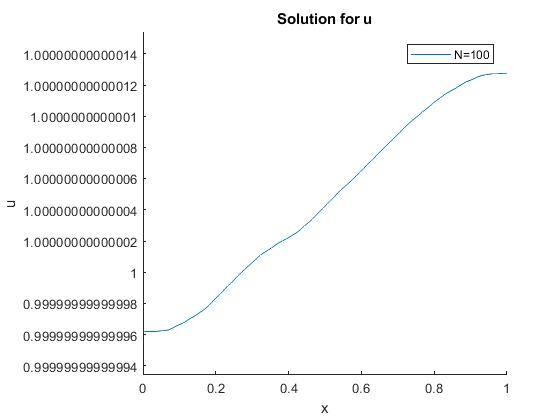
\includegraphics[width=150mm]{1Df1.jpg}
	\caption{showing the calculated u versus x, with N = 100,f(x)=1 \label{overflow}}
\end{figure}

\section{Solution for u}
The final step is to combine all the codes in a main code to solve $Su= \vec{f}$. This code can be found in Appendix A. Previously the S matrix and f vector were computed for $n = 100$. Now $u$ will be calculated for $f(x)=1$, $D=1$, $\nabla = 1$ and $N = 100$. The result of this is plotted in figure(1.2). 


\begin{figure}[ht!]
	\centering
	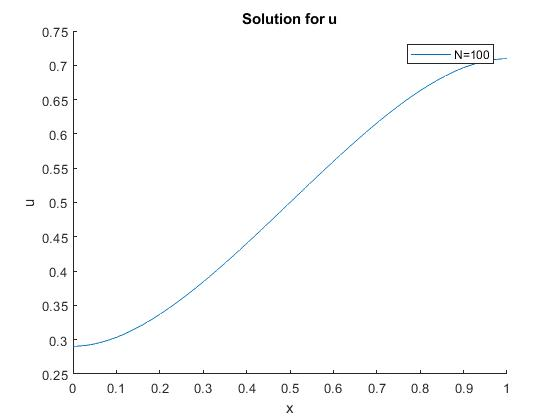
\includegraphics[width=150mm]{1Dfx.jpg}
	\caption{showing the calculated u versus x, with N = 100,f(x)=x 		 \label{overflow}}
\end{figure}



\vfill
\section{Experiment}

The next step is to see what happens when changing f(x) to $f(x)=sin(20x)$ and to see the difference for several values for n ($n=10,20,30,40,80,160)$ 

\vspace{5mm}
\begin{lstlisting}
	function [f] = functionBVP(x)
		f = sin(20*x);
	
		%f = x;
		%f = 1;
	
	end
	
	
	figure 
	hold on
	
	for N_elem = [10 20 40 80 100 160]
	mesh = GenerateMesh(int,N_elem);
	elmat = GenerateTopology(N_elem);
	S = AssembleMatrix( N_elem, lambda, D, mesh, elmat);
	f = AssembleVector( N_elem, mesh, elmat);
	
	x = linspace(int(1),int(2),N_elem);
	
	u = S\f;
	plot(x,u);
	
	legend('N=100')
	title('Solution for u')
	xlabel('x')
	ylabel('u')
	ax.box='on'
	end
	hold off
\end{lstlisting}

\newpage

Figure 1.3

\begin{figure}[ht!]
	\centering
	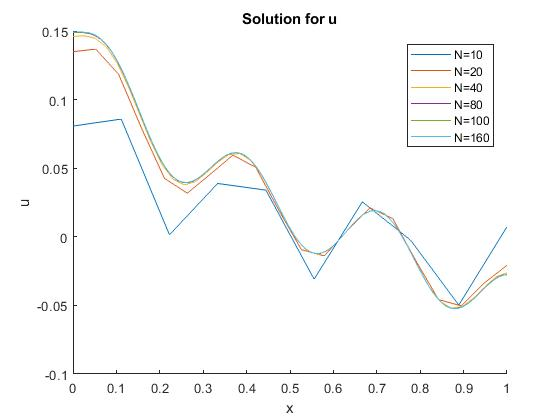
\includegraphics[width=150mm]{1Dfsinx.jpg}
	\caption{showing the calculated u versus x, with N =[10 20 40 80 ]100 160],f(x)=sin(x) \label{overflow}}
\end{figure}


\chapter{2D-case}


The obvious next step after solving a 1 dimensional boundary value problem BVP is to addept the 1D solutions into code to solve a 2 dimensional boundary value problem. To do this a real life problem is going to be solved. In 3rd world countries one of the big issues is the supply of fresh water. One way is to do this is to take square reservoirs, which is a porous medium, with several wells where water is extracted from the subsurface. The water pressure is equal to the hydrostatic pressure. As this is not on an infinite domain, mixed boundary conditions are used. These boundary conditions represent a model for the transfer of the water over the boundary to locations far away. To this extent, a square domain is considered with length 2 in meter: $\Omega= (-1; 1) x (-1; 1)$ with boundary $d\Omega$. Darcy's law for fluid determins the steady state equilibrium of this BVP, given by equation(2.1) :

\begin{equation}
\vec{v}=-\frac{k}{\mu}\nabla p
\end{equation}
\medskip

where p, k, $\mu$ and v, respectively denote the 
fluid pressure, permeability of the porous medium, viscosity of water and the fluid flow velocity. In this BVP the effect of gravity will not play a part as the problem is looked at in 2D. An accompanying assumption is incompressibility, so the extraction wells are treated as point sinks. This assumption can be made as the well its diameter is much smaller than the dimensions of the square reservoir. The extraction wells extract at the same rate in each direction, leading to the following boundary conditions(2.2).


\begin{equation}
	\nabla\cdot\vec{v}=-\sum_{p=1}^{n_{well}}Q_p\delta(\phi(\vec{x}-\phi(\vec{x}_p)=0,(x,y) \epsilon\Omega 
\end{equation}

where $Q_p$ denotes the water extraction rate by well k, which is located at $x_p$. Here $x$ equals $(x;y)$, the spatial coordinates.  We use the convention x = (x; y) to represent the spatial coordinates. The dirac Delta Distribution is characterized by equation(2.3).

\begin{equation}
	\begin{cases} 
		\delta(\vec{x}) = 0,\vec{x} \neq 0 \\ \int_{\Omega}\delta(\vec{x})d\Omega = 1,$  where $\Omega $  contains the origin.$
	\end{cases} 
\end{equation}

\medskip

For this BVP the following boundary condition is considered: 

\begin{equation}
	\vec{v}\cdot\vec{n}=K(p-p^H), \, (x,y)\, \epsilon\,  \partial\Omega
\end{equation}
\bigskip

Here $k$ denotes the transfer rate coefficient of the hormon between the boundary of the domain and its surroundings. The constant $p^H$ represents the hydrostatic pressure. In order to solve this BVP the values needed for all the constants are given in table (2.1).


\begin{table}[ht]
	\caption{Values of input parameters} % title of Table
	\centering % used for centering table
	\begin{tabular}{c c c} % centered columns (3 columns)
		\hline\hline %inserts double horizontal lines
		Symbol & Value & Unit\\ [0.5ex] % inserts table
		%heading
		\hline % inserts single horizontal line
		$Q_p$ & $50$ & $m^2/s$ \\ % inserting body of the table
		$k$ & $10^{-7}$ & $m^2$ \\
		$\mu$ & $1.002\cdot 10^{-3}$ & $Pa\cdot s$ \\
		$K$ & 10 & $m/s$ \\
		$p^H$ & $10^6$ & Pa \\ [1ex] % [1ex] adds vertical space
		\hline %inserts single line
	\end{tabular}
	\label{table:nonlin} % is used to refer this table in the text
\end{table}
\bigskip

In this BVP six wells are considered, which are located at:


\begin{equation}
	\begin{cases} 
		x_p=0.6\cos(\frac{2\pi (p-1)}{5}) \\ x_p=0.6\sin(\frac{2\pi (p-1)}{5})
	\end{cases} 
\end{equation}


\section{Boundary value problem 2D}
The first step to solving these equations using finite elements is to find to find the boundary value problem to solve. This is done by filling in equation(2.1) in both equation 2.2 and the boundary condition(2.4) in order to find the BVP in terms of p:
\vspace{5mm}

BVP:
\begin{equation}
	\begin{cases}
		-\frac{k}{\mu}\triangle\vec{p}=-\sum_{p=1}^{n_{well}}Q_p\delta(\vec{x}-\vec{x}_p)=0,\, \, (x,y) \, \epsilon \, \Omega\\
		-\frac{k}{\mu}\nabla\vec{p}\cdot\vec{n}=-\frac{k}{\mu}\frac{dp}{dn} =K(p-p^H), \, (x,y)\,  \epsilon  \, \partial\Omega
	\end{cases}
\end{equation}

\bigskip

The next step is to compute the weak formulation using the previous found BVP(2.6). By multiplying both sides by $phi(x)$ and integrating both sides over the domain $\Omega$ the weak formulation can be found.

\begin{equation}
	\int_{\Omega}\phi(\vec{x})\nabla\cdot( -\frac{k}{\mu}\nabla\vec{p}) d\Omega =\int_{\Omega}-\sum_{p=1}^{n_{well}}\phi(\vec{x})  Q_p\delta(\vec{x}-\vec{x}_p)
\end{equation}

Using integrating by parts on the left side of equation(2.7) results in:
\begin{equation}
	\int_{\Omega}\nabla\cdot\phi(\vec{x})(-\frac{k}{\mu}\nabla\vec{p})+\frac{k}{\mu}\nabla\phi(\vec{x})\cdot\nabla p d\Omega= -\int_{\Omega}\sum_{p=1}^{n_{well}}\phi(\vec{x}) Q_p\delta(\vec{x}-\vec{x}_p)d\Omega
\end{equation}

Next is to apply Gauss on the first term of the left side.
\begin{equation}
	\int_{d\Omega}\vec{n}\cdot(\phi(\vec{x})(-\frac{k}{\mu}\nabla\vec{p}))d\tau+\int_{\Omega}\frac{k}{\mu}\nabla\phi(\vec{x})\cdot\nabla p d\Omega= -\int_{\Omega}\sum_{p=1}^{n_{well}}\phi(\vec{x}) Q_p\delta(\vec{x}-\vec{x}_p)d\Omega
\end{equation}


Switching the integral and summation on the right side of equation(2.9) and simplifying terms:

\begin{equation}
	\int_{d\Omega}(\phi(\vec{x})(-\frac{k}{\mu}\frac{d\vec{p}}{dn}))\delta\tau+\int_{\Omega}\frac{k}{\mu}\nabla\phi(\vec{x})\cdot\nabla p d\Omega= -\sum_{p=1}^{n_{well}}\int_{\Omega}\phi(\vec{x}) Q_p\delta(\vec{x}-\vec{x}_p)d\Omega
\end{equation}


The right side of equation(2.10) can be simplied using the boundary conditions (equation(2.6)) and the following property into equation(2.12): 

\begin{equation}
	\int_{\Omega}\delta(\vec{x})f(\vec{x})d\Omega \, = \, f(0)	
\end{equation}



\begin{equation}
	\int_{d\Omega}\phi(\vec{x})K(p-p^H)\delta\Gamma+\int_{\Omega}\frac{k}{\mu}\nabla\phi(\vec{x})\cdot\nabla p d\Omega= -\sum_{p=1}^{n_{well}}\phi(\vec{x}_p) Q_p
\end{equation}	

Rearranging equation(2.12) so that the variable parts are on the left and the constant parts on the right leads to the following WF:
\vspace{5mm}


(WF): \begin{equation}
		\begin{cases} 
			$find p $\epsilon \sum =\{p$ $ smooth\}$ Such that:$ \\
			\int_{d\Omega}\phi(\vec{x})Kp\delta\Gamma+\int_{\Omega}\frac{k}{\mu}\nabla\phi(\vec{x})\cdot\nabla p d\Omega= -\sum_{p=1}^{n_{well}}\phi(\vec{x}_p) Q_p +\int_{d\Omega}\phi(\vec{x})Kp^H\delta\Gamma\\ \forall\phi $ $ \epsilon\sum 
		\end{cases}\  
	\end{equation}

To solve the WF the Galerkin equations are applied, where p is replaced by $ \sum_{j=1}^{n}c_i\phi_j $ and  $\phi(x)=\phi_i(x)$ with $i = [1,..,n]$.

\begin{equation}
	\sum_{j=1}^{n}c_i\int_{d\Omega}\phi_i K\phi_j d\Gamma + \int_{\Omega}\frac{k}{\mu}\nabla\phi(x)\cdot\nabla \phi_j d\Omega= -\sum_{p=1}^{n_{well}}\phi(x_p) Q_p +\int_{d\Omega}\phi_i Kp^H\delta\tau
\end{equation}

Equation(2.14) now is of the form $S\vec{c}=\vec{f}$ and like with the 1D problem can be computed. First the element and boundary elements are determined from the Galerkin equations.


\section{Element matrix and element vector}

First the galerkin equation is seperated in its element and boundary components. The element matrix $S^{e_k}_{ij}$ and the element vector $f^{e_k}_i$ are given in equations (2.15) and 2.16 respectively.

\begin{equation}
	S^{e_k}_{ij} = \int_{e_k}\frac{k}{\mu}\nabla\phi_i\cdot\nabla \phi_j d\Omega = (\beta_i\beta_j+\gamma_i\gamma_j)\frac{k}{\mu}\frac{\lvert\triangle e_k\rvert}{2}
\end{equation}

\begin{equation}
	f^{e_k}_i =  -\sum_{p=1}^{n_{well}}\phi(x_p) Q_p
\end{equation}


\section{Boundary matrix and boundary vector}

The boundary matrix $S^{b_l}_{ij}$ and boundary vector $f^{b_l}_i$ can be found in the following equations:

\begin{equation}
	S^{be_l}_{ij} = \int_{b_l} K\phi_i \phi_j dx = K\frac{\lvert be_l\rvert}{6}(1+\delta_{ij})
\end{equation}

\begin{equation}
	f^{be_l}_i = Kp^H\int_{b_l}\phi_i dx = K p^H \frac{\lvert be_l\rvert}{2}
\end{equation}


\section{Cells within an internal element}

To solve the BVP in 2D one of the aspects that need to be determined are whether each internal element contains a cell. This is done by determining whether cell with index $p$ and position $x_p$ is contained within element $e_k$ with vertices $x_{k1}$, $x_{k2}$ and $x_{k3}$. This is done according the following criterion:

\begin{equation}
|\delta(x_p,x_{k2},x_{k3})|+|\delta(x_{k1},x_p,x_{k3})|+|\delta(x_{k1},x_{x2},x_p):
	\begin{cases} 
	=|e_k|,\, x_p\, \in, \vec{e_k}\\ 
	>|e_k|,\, x_p\, \notin\,\vec{e_k}
	\end{cases} 
\end{equation}

In the criterion $\delta(x_p,x_q,x_r)$ denotes the triangle with vertices $x_p$, $x_q$ and $x_r$, where $|\delta(x_{k1},x_{k2},x_{k3})$ denote its area. The triangular element $k$ is given by $e_k=\delta(x_{k1},x_{k2},x_{k3})$ with vertices  $x_1$, $x_2$ and $x_3$ and $\vec{e_k}$ includes the boundary of element $e_k$. To solve this BVP a certan tolerance has to be accounted for in the Matlab code.

\section{Generating MATLAB code}

Similar as with the 1D BVP, code is written in order to generate a mesh, element matrix, element vector, boundary element matrix and boundary element vector. These codes can be found in appendix B.1 through B.6. 





\section{Assignment 8}

Now Darcy's law is used to compute the velocity in both directions, by implementing the found WF(equation (2.13)) and the Galerkin equations in the resulting system of linear equations(2.20).

\begin{equation}
 M\vec{v_x}=C_x\vec{p},\,\,\, M\vec{v_y}=C_y\vec{p}
\end{equation}

In order to find $\vec{v_x}$ and $\vec{v_y}$ equations(2.20) need to be solved. First writing out the x and y parts of the velocity gives:

\begin{equation}
\vec{v}=-\frac{k}{\mu}\nabla p
\end{equation}

\begin{equation}
\vec{v}_x=-\frac{k}{\mu}\frac{dp}{dx}
\end{equation}


\begin{equation}
\vec{v}_y=-\frac{k}{\mu}\frac{dp}{dy}
\end{equation}

Equation(2.24) shows the relation between $\vec{v}$ and pressure p.

\begin{equation}
\vec{v}\cdot\vec{n}=k(p-p^H)\text{ on }d\Omega
\end{equation}

This relation is used to rewrite equations(2.22 and 2.23):

\begin{equation}
v_x(x=-1)=-k(p-p^H)
\end{equation}


\begin{equation}
v_x(x=1)=k(p-p^H)
\end{equation}


\begin{equation}
v_y(y=-1)=-k(p-p^H)
\end{equation}


\begin{equation}
v_y(y=1)=k(p-p^H)
\end{equation}

The Galerkin approach is used again to solve the equations by approximating $v_x$.

\begin{equation}
v_x \approx v^{(n)}_x=\sum_{j=1}^{n}c_j \phi_j
\end{equation}

Here $\phi(\vec{x})=\phi (\vec{x})_i$. Filling equations(2.29) and $\phi(\vec{x})_i$ in the exuations for $v_x$ 


\begin{equation}
\int_{\Omega}\phi v_x d\Omega=-\frac{k}{\mu}\int_{\Omega}\phi\frac{dp}{dx}d\Omega
\end{equation}

Partial integration is applied on the right side term.
\begin{equation}
\int_{\Omega}\phi v_x d\Omega=  -\frac{k}{\mu}\{\int_{\Omega}\frac{d}{dx}(\phi p)-p\frac{d\phi}{x}d\Omega\}
\end{equation}

Rewriting the integral:

\begin{equation}
 \int_{\Omega}-\frac{k}{\mu}\frac{d\phi p}{dx}dxdy=\int_{-1}^{1}=-\frac{k}{\mu}[\phi p]dy
\end{equation}

Evaluating the right side of equation(2.31) by filling in the previous conditions for specific points (1,1) and (-1,-1):
\begin{equation}
=\int_{-1}^{1}-\frac{k}{\mu}(\phi(x=1,y)p(x=1,y))-\frac{k}{\mu}(\phi(x=-1)p(x=-1,y))dy
\end{equation}

Simplifying the equation:

\begin{equation}
=\int_{d\Omega_3}-\frac{k}{\mu}\phi pdy+\int_{d\Omega_1}\frac{k}{\mu}\phi pdy
\end{equation}

Now the total combined equation found is:
\begin{equation}
\int_{\Omega}\phi v_x = -\frac{k}{\mu}\{\int_{\Omega}\frac{d}{dx}(\phi p)-p\frac{d\phi}{dx}d\Omega\}
\end{equation}


Find $v_x$ stationary:

\begin{equation}
\int_{\Omega}\phi v_x = \frac{k}{\mu}\{\int_{d\Omega_3}-\phi pdy+\int_{d\Omega_1}\phi pdy+\int_{\Omega}p\frac{\phi_i}{dx}d\Omega\}
\end{equation}


Again applying the Galerkin equations to (2.36) the following conditions are found(2.38).

\begin{equation}
\phi(\vec{x})=\phi(\vec{x})_i \hspace{1cm}v_x\approx v^{(n)}_x = \sum_{j=1}^{n}c_j\phi(\vec{x})_j
\end{equation}


\begin{equation}
\text{on}\,
\begin{cases}
d\Omega_3:\, -v_x=k(p-p^H) \,\rightarrow\, p=-\frac{v_x}{k}+p^H\\
d\Omega_1:\,\,\,\,\, v_x=k(p-p^H) \,\rightarrow\, p=\frac{v_x}{k}+p^H
\end{cases}
\end{equation}

Now writing the equation where $v_x$ is filled in so that an equation is found that depends on $p$. 

\begin{equation}
	\int_{\Omega}\phi v_x d\Omega + \int_{d\Omega_3}-\frac{k}{\mu}\frac{1}{k}\phi v_xdy + \int_{d\Omega_1}-\frac{k}{\mu}\frac{1}{k}\phi v_x dy 
	= \int_{d\Omega_3}-\frac{k}{\mu}\phi p^H dy +\int_{d\Omega_1}\frac{k}{\mu}\phi p^H dy + \int_{\Omega}\frac{k}{\mu}p\frac{d\phi}{dx}d\Omega
\end{equation}

For the right side of equation(2.39) the galerkin equations are filled in to find a 
$\phi(\vec{x})=\phi(\vec{x})_i$\,\,\,\,  $v_x\approx \sum_{j=1}^{n}c_j\phi(\vec{x})_j$  \,\,\,\,$\phi(\vec{x})=\alpha_i+\beta_i x+\gamma_i y$

\begin{equation}
\sum_{j=1}^{n}c_j
\{\int_{\Omega}\phi_i\phi_j d\Omega +\int_{d\Omega_3}-\frac{k}{\mu}\frac{1}{k}\phi_i\phi_j dy + \int_{d\Omega_1}-\frac{k}{\mu}\frac{1}{k}\phi_i\phi_j dy \}
\end{equation}

\begin{equation}
\sum_{j=1}^{n}c_j
\{\int_{d\Omega_3}-\frac{k}{\mu}\phi_i p^H dy +\int_{d\Omega_1}\frac{k}{\mu}\phi_i p^H dy + \int_{\Omega}\frac{k}{\mu}p\frac{d\phi_i}{dx}d\Omega\}
\end{equation}



Applying Newton-Cotes theorem and ~ , the element matrix(2.42), boundary element matrix(2.43), element vector(2.44) and boundary element vector(2.45) is found.

\begin{equation}
S^{e_k}_{ij}=\int_{e_k}\phi_i\phi_j = \frac{\lvert\triangle_{ek}\rvert}{24}
\end{equation}

\begin{equation}
S^{be_l}_{ij}=\int_{be_l}-\frac{k}{\mu}\phi_i\phi_j dy = \frac{k}{\mu}\frac{1}{k}\frac{\lvert be_l\rvert}{6}(1+\delta_{ij})
\end{equation}

\begin{equation}
f^{e_n}_{i} = \int_{e_n}\frac{k}{\mu}p\beta_i d\Omega = \frac{k}{\mu}\beta_i\sum_{m=\in\{k_1,k_2,k_3\}} p(\vec{x}_m) \frac{\lvert \triangle e_n\rvert}{6}
\end{equation}

\begin{equation}
f^{be_l}_{i}=\int_{be_l}\pm \frac{k}{\mu}\phi_ip^H dy = \pm \frac{k}{\mu}p^H \frac{\lvert be_l\rvert}{2}
\end{equation}


\begin{figure}[ht!]
	\centering
	\includegraphics[width=150mm]{meshgrid2D.jpg}
	\caption{caption
 \label{overflow}}
\end{figure}

\begin{figure}[ht!]
	\centering
	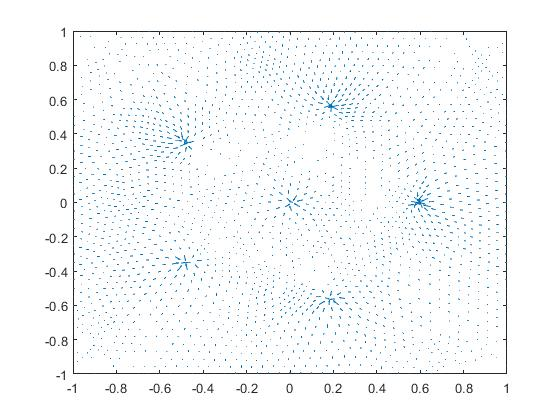
\includegraphics[width=150mm]{2Dvarrows.jpg}
	\caption{caption
	\label{overflow}}
\end{figure}

\begin{figure}[ht!]
	\centering
	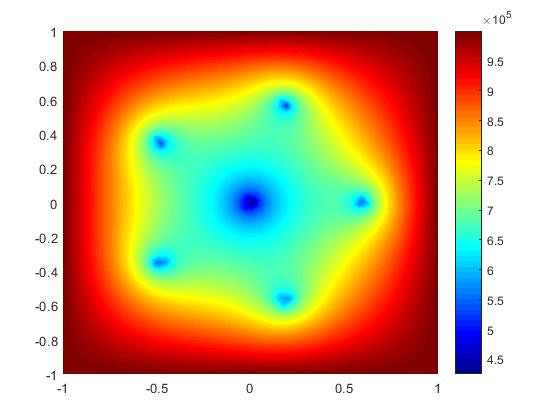
\includegraphics[width=150mm]{2Dvheat.jpg}
	\caption{caption
	\label{overflow}}
\end{figure}

\begin{figure}[ht!]
	\centering
	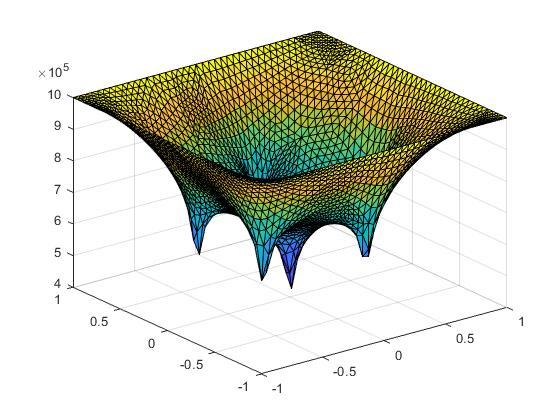
\includegraphics[width=150mm]{3Dv.jpg}
	\caption{caption
	\label{overflow}}
\end{figure}

\section{Assignment 9}

%Perform various simulations where you let the transfer coeficient K range between 0.00001 and 10000. Show the contour plots, and give the values of the minimal pressure (which is important from an engineering point of view). Explain your results.





\section{Assignment 10}

What happens if K = 0? Explain the results.



\newpage

\appendix

\begin{appendices}
\chapter{1D-case full script}


\begin{lstlisting}
clear all
close all

%%Finite Element 1D
%% Parameters

N_elem = 100; %Number of elements
int = [0,1]; %Interval
lambda = 1;
D = .1;

%% Mesh & Topology

mesh = GenerateMesh(int,N_elem);
elmat = GenerateTopology(N_elem); %1D topology!!

%% Assemble Matrix & Vector

S = AssembleMatrix( N_elem, lambda, D, mesh, elmat);
f = AssembleVector( N_elem, mesh, elmat);

%% Calculate u
x = linspace(int(1),int(2),N_elem);

u = S\f;

hold on
plot(x,u); 
legend('N=100')
title('Solution for u')
xlabel('x')
ylabel('u')
ax.box='on'
hold off


% For this part change the function in functionBVP.m to 'f = sin(20*x)'

figure 
hold on

for N_elem = [10 20 40 80 100 160]
	mesh = GenerateMesh(int,N_elem);
	elmat = GenerateTopology(N_elem);
	S = AssembleMatrix( N_elem, lambda, D, mesh, elmat);
	f = AssembleVector( N_elem, mesh, elmat);

	x = linspace(int(1),int(2),N_elem);

	u = S\f;
	plot(x,u);


end

legend('N=10','N=20','N=40','N= 80','N=100','N=160')
title('Solution for u')
xlabel('x')
ylabel('u')
ax.box='on'
hold off
\chapter{2D-case full script}




\end{lstlisting}

\chapter{2D-case}


\section{Generate mesh}
\begin{lstlisting}
clear all

Geometry = 'squareg'; 

DiffCoeff = 1;
h_transfer = 1;
u_inf = 1;


% Geometry = 'squareg'; % gives square [-1,1] x [-1,1]
% Geometry = 'circleg'; % gives unit circle centered at origin
% Geometry = 'lshapeg'; % gives L-shape

[p,e,t] = initmesh(Geometry);
[p,e,t] = refinemesh(Geometry,p,e,t); % gives gridrefinement
[p,e,t] = refinemesh(Geometry,p,e,t); % gives second gridrefinement
%[p,e,t] = refinemesh(Geometry,p,e,t); % gives third gridrefinement
pdemesh(p,e,t); % plots the geometry and mesh

x = p(1,:); y = p(2,:);
n = length(p(1,:));

elmat = t(1:3,:);
elmat = elmat';
elmatbnd = e(1:2,:);
elmatbnd = elmatbnd';
% h
topology = 3; topologybnd = 2;
\end{lstlisting}




\section{Generate element matrix}
\begin{lstlisting}
clear xc
clear yc
clear Selem

for index1 = 1:topology
xc(index1) = x(elmat(i,index1));
yc(index1) = y(elmat(i,index1));
end;

Delta = det([1 xc(1) yc(1);1 xc(2) yc(2);1 xc(3) yc(3)]);
B_mat = [1 xc(1) yc(1);1 xc(2) yc(2);1 xc(3) yc(3)] \  eye(3);

alpha = B_mat(1,1:3);
beta  = B_mat(2,1:3);
gamma = B_mat(3,1:3);

for index1 = 1:topology
for index2 = 1:topology
if ~exist('u','var')
Selem(index1,index2) =
abs(Delta)/2*(k/mu)*(beta(index1)*beta(index2)+gamma(index1)*gamma(index2));
else
Selem(index1,index2) = abs(Delta)/24;
end
end;
end;
\end{lstlisting}

\section{Generate element vector}
\begin{lstlisting}
clear xc
clear yc
clear felem

for index1=1:topology
xc(index1) = x(elmat(i,index1));
yc(index1) = y(elmat(i,index1));
end;

Delta = det([1 xc(1) yc(1);1 xc(2) yc(2);1 xc(3) yc(3)]);
B_mat = [1 xc(1) yc(1);1 xc(2) yc(2);1 xc(3) yc(3)] \  eye(3);

alpha = B_mat(1,1:3);
beta  = B_mat(2,1:3);
gamma = B_mat(3,1:3);

felem = zeros(1,topology);

% for N = 1:N_wells
%     Delta_23 = det([1 xp(N) yp(N);1 xc(2) yc(2);1 xc(3) yc(3)]);
%     Delta_13 = det([1 xc(1) yc(1);1 xp(N) yp(N);1 xc(3) yc(3)]);
%     Delta_12 = det([1 xc(1) yc(1);1 xc(2) yc(2);1 xp(N) yp(N)]);
%     
%     if Delta + epsilon1*Delta >= abs(Delta_23) + abs(Delta_13) 
+ abs(Delta_12) || Delta - epsilon1*Delta >= abs(Delta_23)
+ abs(Delta_13) + abs(Delta_12) ;
%         N_Test = N_Test + 1;
%         for index1 = 1:topology
%             felem(index1) = felem(index1) +
			-Qp*(1-abs(beta(index1))*abs(xc(index1)-
			xp(index1))-abs(gamma(index1))*abs(yc(index1)-yp(index1)));
%             
%         end
%         
%     i
% % Components of f are zero except for those elements with a well! So no
% % other contributions!
% %     else        
% %         for index1 = 1:topology
% %         global_index = elmat(N,index1);
% %         
% %         
% %         end
%     end
% end
if ~exist('u','var')
for N = 1:N_wells
for index3 = 1:topology
phi_p(index3) = alpha(index3) + beta(index3)*xp(N) 
+ gamma(index3)*yp(N);
end

if (phi_p(1) <= 1) && (phi_p(1) >= 0) && (phi_p(2) <= 1) && (phi_p(2) 
>= 0) && (phi_p(3) <= 1) && (phi_p(3) >= 0);
for index1 = 1:topology
phi_p
felem(index1) = felem(index1) +
-Qp*phi_p(index1); %*(1-abs(beta(index1))*abs(xc(index1)
-xp(index1))-abs(gamma(index1))*abs(yc(index1)-yp(index1))) ;
felem
end
i

N_Test = N_Test + 1;
% Components of f are zero except for those elements with a well! So no
% other contributions!
%     else        
%         for index1 = 1:topology
%         global_index = elmat(N,index1);
%         
%         
%         end
end
end
else
switch direction
case 1 % x direction
for index1 = 1:topology
felem(index1) = felem(index1) +
(k/mu)*(abs(Delta)/6)*beta(index1)*(u(elmat(i,1))+u(elmat(i,2))+u(elmat(i,3)));
end

case 2 % y direction
for index1 = 1:topology
felem(index1) = felem(index1) +
(k/mu)*(abs(Delta)/6)*gamma(index1)*(u(elmat(i,1))+u(elmat(i,2))+u(elmat(i,3)));
end
end
end
\end{lstlisting}





\section{Generate Boundary matrix}

\begin{lstlisting}
clear xc
clear yc
clear BMelem

for index1=1:topologybnd
xc(index1) = x(elmatbnd(i,index1));
yc(index1) = y(elmatbnd(i,index1));
end;

lek = sqrt((xc(2)-xc(1))^2 + (yc(2)-yc(1))^2);

for index1=1:topologybnd
if ~exist('u', 'var')
BMelem(index1,index1) = K*lek/2;  % NC used! not HB!!
else

BMelem(index1,index1) = -(k/(mu*K))*lek/6;
end
end;
\end{lstlisting}



\section{Generate boundary element vector:}

\begin{lstlisting}
clear xc
clear yc
clear bfelem

for index1 = 1:topologybnd
xc(index1) = x(elmatbnd(i,index1));
yc(index1) = y(elmatbnd(i,index1));
end;

lek = sqrt((xc(2)-xc(1))^2+(yc(2)-yc(1))^2);

if ~exist('u','var')
for index1 = 1:topologybnd
bfelem(index1) = K*pH*lek/2*u_inf;   %what is u_inf?
end;
else
for index1 = 1:topologybnd
bfelem(index1) = ((k*pH)/mu)*lek/2*u_inf;   %what is u_inf?
%         bfelem(index1) = -(k/mu)*lek/6*u(elmat(i,ind1));
end
end
\end{lstlisting}

\section{Buildmatrices and vectors}

\begin{lstlisting}
% This routine constructs the large matrices and vector.
% The element matrices and vectors are also dealt with.
% First the internal element contributions
% First Initialisation of large discretisation matrix, right-hand side vector

% Treatment of the internal (triangular) elements

if ~exist('u', 'var')  

S 		= sparse(n,n); % stiffness matrix

f 		= zeros(n,1); % right-hand side vector

for i = 1:length(elmat(:,1)) % for all internal elements
GenerateElementMatrix; % Selem	
for ind1 = 1:topology
for ind2 = 1:topology
S(elmat(i,ind1),elmat(i,ind2))	= S(elmat(i,ind1),elmat(i,ind2)) + Selem(ind1,ind2);
end;
end;

GenerateElementVector; % felem
for ind1 = 1:topology
f(elmat(i,ind1)) = f(elmat(i,ind1)) + felem(ind1);
end;
end;

% Next the boundary contributions

for i = 1:length(elmatbnd(:,1)); % for all boundary elements extension of mass matrix M and element vector f
GenerateBoundaryElementMatrix; % BMelem
for ind1 = 1:topologybnd
for ind2 = 1:topologybnd
S(elmatbnd(i,ind1),elmatbnd(i,ind2)) = S(elmatbnd(i,ind1),elmatbnd(i,ind2)) + BMelem(ind1,ind2);
end;
end;
GenerateBoundaryElementVector; % bfelem   
for ind1 = 1:topologybnd
f(elmatbnd(i,ind1)) = f(elmatbnd(i,ind1)) + bfelem(ind1);
end;
end;

else

Sx 		= sparse(n,n); % stiffness matrix

fx 		= zeros(n,1); % right-hand side vector

left_nodes = find(p(1,:) == -1); 
top_nodes = find(p(2,:) == 1);
right_nodes = find(p(1,:) == 1);
bottom_nodes = find(p(2,:) == -1);

bnd1_nodes = ismember(elmatbnd,left_nodes);
bnd1 = find(bnd1_nodes(:,1) == 1 & bnd1_nodes(:,2) == 1);

bnd2_nodes = ismember(elmatbnd,top_nodes);
bnd2 = find(bnd2_nodes(:,1) == 1 & bnd2_nodes(:,2) == 1);

bnd3_nodes = ismember(elmatbnd,right_nodes);
bnd3 = find(bnd3_nodes(:,1) == 1 & bnd3_nodes(:,2) == 1);

bnd4_nodes = ismember(elmatbnd,bottom_nodes);
bnd4 = find(bnd4_nodes(:,1) == 1 & bnd4_nodes(:,2) == 1);


direction = 1;

for i = 1:length(elmat(:,1)) % for all internal elements
GenerateElementMatrix; % Selem	
for ind1 = 1:topology
for ind2 = 1:topology
if elmat(i,ind1) == elmat(i,ind2)
Sx(elmat(i,ind1),elmat(i,ind2))	= Sx(elmat(i,ind1),elmat(i,ind2)) + 2*Selem(ind1,ind2);
else
Sx(elmat(i,ind1),elmat(i,ind2))	= Sx(elmat(i,ind1),elmat(i,ind2)) + Selem(ind1,ind2);
end
end;
end;
GenerateElementVector; % felem
for ind1 = 1:topology
fx(elmat(i,ind1)) = fx(elmat(i,ind1)) + felem(ind1);
end;
end;

% Next the boundary contributions



for j = 1:length(bnd1); % left boundary
i = bnd1(j);
GenerateBoundaryElementMatrix; % BMelem
for ind1 = 1:topologybnd
for ind2 = 1:topologybnd
if elmatbnd(i,ind1) == elmatbnd(i,ind2)
Sx(elmatbnd(i,ind1),elmatbnd(i,ind2)) = Sx(elmatbnd(i,ind1),elmatbnd(i,ind2)) + 2*BMelem(ind1,ind2);
else
Sx(elmatbnd(i,ind1),elmatbnd(i,ind2)) = Sx(elmatbnd(i,ind1),elmatbnd(i,ind2)) + BMelem(ind1,ind2);
end;
end
end;
GenerateBoundaryElementVector; % bfelem   
for ind1 = 1:topologybnd
fx(elmatbnd(i,ind1)) = fx(elmatbnd(i,ind1)) + bfelem(ind1);
end;
end;

for j = 1:length(bnd3); % right boundary
i = bnd3(j);
GenerateBoundaryElementMatrix; % BMelem
for ind1 = 1:topologybnd
for ind2 = 1:topologybnd
if elmatbnd(i,ind1) == elmatbnd(i,ind2)
Sx(elmatbnd(i,ind1),elmatbnd(i,ind2)) = Sx(elmatbnd(i,ind1),elmatbnd(i,ind2)) + 2*BMelem(ind1,ind2);
else
Sx(elmatbnd(i,ind1),elmatbnd(i,ind2)) = Sx(elmatbnd(i,ind1),elmatbnd(i,ind2)) + BMelem(ind1,ind2);
end;
end
end;
GenerateBoundaryElementVector; % bfelem   
for ind1 = 1:topologybnd
fx(elmatbnd(i,ind1)) = fx(elmatbnd(i,ind1)) - bfelem(ind1);
end;
end;

direction = 2;

Sy 		= sparse(n,n); % stiffness matrix

fy 		= zeros(n,1); % right-hand side vector

for i = 1:length(elmat(:,1)) % for all internal elements
GenerateElementMatrix; % Selem	
for ind1 = 1:topology
for ind2 = 1:topology
if elmat(i,ind1) == elmat(i,ind2)
Sy(elmat(i,ind1),elmat(i,ind2))	= Sy(elmat(i,ind1),elmat(i,ind2)) + 2*Selem(ind1,ind2);
else
Sy(elmat(i,ind1),elmat(i,ind2))	= Sy(elmat(i,ind1),elmat(i,ind2)) + Selem(ind1,ind2);
end
end;
end;
GenerateElementVector; % felem
for ind1 = 1:topology
fy(elmat(i,ind1)) = fy(elmat(i,ind1)) + felem(ind1);
end;
end;

% Next the boundary contributions



for j = 1:length(bnd2); % left boundary
i = bnd2(j);
GenerateBoundaryElementMatrix; % BMelem
for ind1 = 1:topologybnd
for ind2 = 1:topologybnd
if elmatbnd(i,ind1) == elmatbnd(i,ind2)
Sy(elmatbnd(i,ind1),elmatbnd(i,ind2)) = Sy(elmatbnd(i,ind1),elmatbnd(i,ind2)) + 2*BMelem(ind1,ind2);
else
Sy(elmatbnd(i,ind1),elmatbnd(i,ind2)) = Sy(elmatbnd(i,ind1),elmatbnd(i,ind2)) + BMelem(ind1,ind2);
end;
end
end;
GenerateBoundaryElementVector; % bfelem   
for ind1 = 1:topologybnd
fy(elmatbnd(i,ind1)) = fy(elmatbnd(i,ind1)) - bfelem(ind1);
end;
end;

for j = 1:length(bnd4); % right boundary
i = bnd4(j);
GenerateBoundaryElementMatrix; % BMelem
for ind1 = 1:topologybnd
for ind2 = 1:topologybnd
if elmatbnd(i,ind1) == elmatbnd(i,ind2)
Sy(elmatbnd(i,ind1),elmatbnd(i,ind2)) = Sy(elmatbnd(i,ind1),elmatbnd(i,ind2)) + 2*BMelem(ind1,ind2);
else
Sy(elmatbnd(i,ind1),elmatbnd(i,ind2)) = Sy(elmatbnd(i,ind1),elmatbnd(i,ind2)) + BMelem(ind1,ind2);
end;
end
end;
GenerateBoundaryElementVector; % bfelem   
for ind1 = 1:topologybnd
fy(elmatbnd(i,ind1)) = fy(elmatbnd(i,ind1)) + bfelem(ind1);
end;
end;
end

\end{lstlisting}

\section{Compute u and $v_x$/$v_y$}


\begin{lstlisting}
% Construction of linear problem

BuildMatricesandVectors;

% Solution of linear problem

u = S \ f;

BuildMatricesandVectors;

vx = Sx \ fx;
vy = Sy \ fy;
\end{lstlisting}

\section{Full script}
\begin{lstlisting}
close all
clear all

%% 2D Assignment
% Lab Assignment 7

%% Create Mesh
WI4243Mesh

%% Parameters

Qp = 50;            % [m^2/s]
k = 10^-7;          % [m^2]
mu = 1.002*10^-3;   % [Pa*s]
K = 10000;             % [m/s]
pH = 10^6;          % [Pa]
N_wells = 6;        % number of wells

epsilon1 = 0.03;
N_Test = 0;
%% Coordinates of wells

for i = 1:N_wells-1;
xp(i) = 0.6*cos((2*pi)*(i-1)/(N_wells-1));
yp(i) = 0.6*sin((2*pi)*(i-1)/(N_wells-1));
end

xp(N_wells) = 0;
yp(N_wells) = 0;
clear i;


%% Compute Problem
WI4243Comp

%% Post
WI4243Post

%% Velocity part


\end{lstlisting}

\end{appendices}

\end{document}




	